%%%%%%%%%%%%%%%%%%%%%%%%%%%%%%%%%%%%%%%%%%%%%%%%%%%%%%%%%%%%%%%%
%%%%%%%%%%%%%%%%%%%%%%%%%%%%%%%%%%%%%%%%%%%%%%%%%%%%%%%%%%%%%%%%
%%%%
%%%% This text file is part of the source of slides for
%%%% `Introduction to High-Performance Scientific Computing'
%%%% by Victor Eijkhout, copyright 2012-2021
%%%%
%%%%%%%%%%%%%%%%%%%%%%%%%%%%%%%%%%%%%%%%%%%%%%%%%%%%%%%%%%%%%%%%
%%%%%%%%%%%%%%%%%%%%%%%%%%%%%%%%%%%%%%%%%%%%%%%%%%%%%%%%%%%%%%%%

\begin{numberedframe}{Graph algorithms}
  \begin{itemize}
  \item Traditional: search, shortest path, connected components
  \item New: centrality
  \end{itemize}
\end{numberedframe}

\begin{numberedframe}{Traditional use of graph algorithms}
  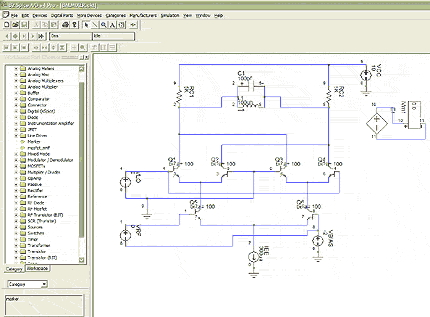
\includegraphics[scale=.6]{schematic}
\end{numberedframe}

\begin{numberedframe}{1990s use of graph algorithms}
  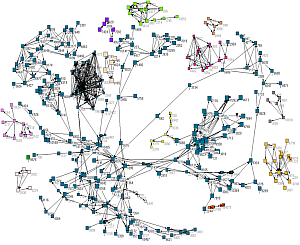
\includegraphics[scale=.8]{lsggraph}
\end{numberedframe}

\begin{numberedframe}{2010 use of graph algorithms}
  
\includegraphics[scale=.1]{fbgraph}
\end{numberedframe}

\begin{numberedframe}{2010 use of graph algorithms}
  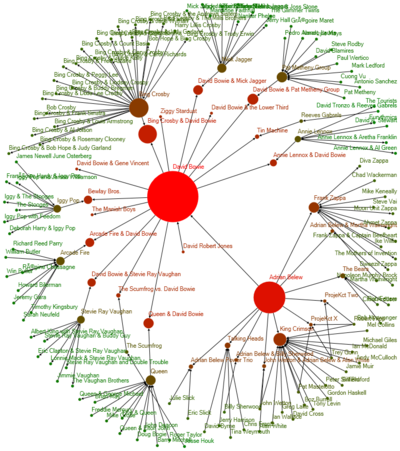
\includegraphics[scale=.7]{bowie_graph}
\end{numberedframe}

\begin{numberedframe}{Shortest distance algorithm}
  Given node~$s$:
  \[ d\colon v\mapsto d(s,v) \]
\begin{displayalgorithm}
  \Input{A graph, and a starting node~$s$}
  \Output{A function $d(v)$ that measures the distance from $s$ to~$v$}
  Let $s$ be given, and set $d(s)=0$\;
  Initialize the finished set as $U=\{s\}$\;
  Set $c=1$\;
  \While{not finished}{
    Let $V$ the neighbours of $U$ that are not themselves in $U$\;
    \If{$V=\emptyset$}{We're done}\Else{
    Set $d(v)=c+1$ for all $v\in V$.\;
    $U\leftarrow U\cup V$\;
    Increase $c\leftarrow c+1$
    }
  }
\end{displayalgorithm}
\end{numberedframe}

\begin{numberedframe}{Level sets}
  The steps in the algorithm are `level sets':

  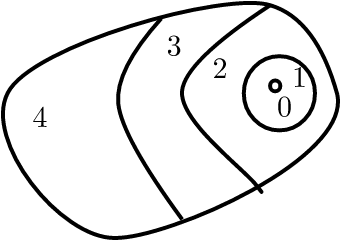
\includegraphics[scale=.4]{levelset}  
\end{numberedframe}

\begin{numberedframe}{Computational characteristics}
  \begin{itemize}
  \item Uses a queue: central storage
  \item Parallelism not self-evident
  \item Flexible assignment of work to processors, so no locality
  \end{itemize}
\end{numberedframe}

\begin{numberedframe}{Example}
  \includegraphics[scale=.1]{dijkstra/graph}
\end{numberedframe}

\begin{numberedframe}{Level 1}
  \includegraphics[scale=.1]{dijkstra/dijkstra1}
\end{numberedframe}

\begin{numberedframe}{Level 2}
  \includegraphics[scale=.1]{dijkstra/dijkstra2}
\end{numberedframe}

\begin{numberedframe}{Level 3}
  \includegraphics[scale=.1]{dijkstra/dijkstra3}
\end{numberedframe}

\begin{numberedframe}{Matrix view}
  \includegraphics[scale=.1]{dijkstra/matrix}
\end{numberedframe}

\begin{numberedframe}{Level 1}
  \includegraphics[scale=.1]{dijkstra/mvp1}
\end{numberedframe}

\begin{numberedframe}{Level 2}
  \includegraphics[scale=.1]{dijkstra/mvp2}
\end{numberedframe}

\begin{numberedframe}{summing up}
  \hbox\bgroup
  \includegraphics[scale=.09]{dijkstra/mvpsum}
  \includegraphics[scale=.09]{dijkstra/mvpops}
  \egroup
\end{numberedframe}



\begin{comment}
\begin{numberedframe}{Matrix formulation}
Let 
\[ x_i = 
\begin{cases}
  1&i=s\\ \infty&\hbox{otherwise}
\end{cases}
\]
Let $x$ zero except in~$i$,\\
then $x^tG$ nonzero in $j$ if there is an edge $(i,j)$
\end{numberedframe}

\begin{numberedframe}{Matrix algorithm}
  
Define a product as
\[ y^t=x^tG\equiv \forall_i\colon
  (y^t)_j = \min_{i\colon G_{ij}\not=0} x_i+1,
\]
Iterate
\[ x,x^tG,x^tG^2,\ldots \]
After $k$ (diameter) iterations $(x^tG^k)_i$ is the distance $d(s, i)$.
\end{numberedframe}

\begin{numberedframe}{Single Source Shortest Path}
  Similar to previous, but non-unit edge weights
\begin{displayalgorithm}
  Let $s$ be given, and set $d(s)=0$\;
  Set $d(v)=\infty$ for all other nodes~$v$\;
  \For{$|E|-1$ times}{
    \For{all edges $e=(u,v)$}{
      Relax: \If{$d(u)+w_{uv}<d(v)$}{Set $d(v)\leftarrow d(u)+w_{uv}$}
    }
  }
\end{displayalgorithm}
\[ y^t=x^tG\equiv \forall_i\colon
  y_j = \min\bigl\{ x_j, \min_{i\colon G_{ij}\not=0} \{x_i+g_{ij}\} \bigr\},
\]
\end{numberedframe}
\end{comment}

\begin{numberedframe}{All-pairs shortest path}
\begin{equation}
  \Delta_{k+1}(u,v) = \min\bigl\{ \Delta_k(u,v),
  \Delta_k(u,k)+\Delta_k(k,v) \bigr\}.
  \label{eq:floyd-allpairs}
\end{equation}

Algebraically:
\begin{displayalgorithm}
  \For {$k$ from zero to $|V|$} {
    $D\leftarrow D._{\min} \bigl[D(:,k) \mathbin{\min\cdot_+} D(k,:) \bigr]$
  }
\end{displayalgorithm}
Similarity to Gaussian elimination  
\end{numberedframe}

\begin{numberedframe}{Pagerank}
  $T$ stochastic: all rowsums are~$1$.

  Prove $x^te=1\Rightarrow x^tT=1$

  Pagerank is essentially a power method: $x^t,x^tT,x^tT^2,\ldots$
  modeling page transitions.

  Prevent getting stuck with random jump: \[ x^t\leftarrow sx^tT+(1-s)e^t \]

  Solution of linear system: \[ x^t(I-sT)=(1-s)e^t \]
  Observe \[ (I-sT)\inv = I+sT+s^2T^2+\cdots \]
\end{numberedframe}

\begin{numberedframe}{`Real world' graphs}
  \begin{itemize}
  \item Graphs imply sparse matrix vector product
  \item \ldots but the graphs are unlike PDE graphs
  \item differences:
    \begin{itemize}
    \item low diameter \item high degree \item power law
    \end{itemize}
  \item treat as random sparse: use dense techniques
  \item 2D matrix partitioning: each block non-null, but sparse
  \end{itemize}  
\end{numberedframe}

\begin{numberedframe}{Parallel treatment}
  \begin{itemize}
  \item Intuitive approach: partitioning of nodes
  \item equivalent to 1D matrix distribution
  \item not scalable $\Rightarrow$ 2D distribution
  \item equivalent to distribution of edges
  \item unlike with PDE graphs, random placement may actually be good
  \end{itemize}
\end{numberedframe}
